\documentclass[11pt]{article}
\usepackage[margin=0.85in]{geometry}
\usepackage[T1]{fontenc}
\usepackage{lmodern,amsmath,amssymb,graphicx,booktabs,hyperref,enumitem}
\usepackage[font=small]{caption}
\graphicspath{{assets/}}
\newcommand{\kb}{k_{\rm B}}
\title{Overview: energy-conditioned vacancy generation\\
\large Adaptive labels, latent information, and entropy sampling}
\author{Ricardo Silva Buarque \quad Beihao Gu \quad Varad Kottawar}
\date{November 12--13, 2026}
\begin{document}
\maketitle
Observed-range labels improve first-round balanced sampling by roughly six
percentage points, but a second acquired batch does not sustain that gain
against its matched continuation. The follow-up recovers a similar gain by
relabeling H0 alone. This identifies conditioning and its induced class
weighting as important parts of the result; adding configurations is not a
uniform benefit. Most of the gain is in HIGH-class fidelity, rather than
low-energy discovery.

The tested CVAEs do not establish a primary sampling advantage over the
no-latent autoregressive model. Their deterministic posterior means retain
a recoverable vacancy-ordering fingerprint. A fixed-condition random-encoder
control also contains this fingerprint, so recovery alone does not show
that training discovered it. That information does not become reliable
control of generated structures. In the illustrated fixed condition, tiny
mean variations coexist with nearly unit-scale posterior noise; a readable
mean scatter and a useful sampled latent are different outcomes.

Entropy estimation needs a different sampling objective. On the complete
12-site lattice, correct orbit multiplicities and proposal probabilities
are essential. Training toward a 1,000\,K Boltzmann target reduces the
equal-composition entropy MAE from 0.01310 to 0.00420\,$\kb$/cell for UMA
and from 0.01371 to 0.00313 for MACE. The same proposals are worse than
uniform sampling at 5,000\,K. Histogram flattening also does not establish
energy-bin convergence in the Wang--Landau calculation.

These findings concern fixed O3-derived vacancy lattices and the supplied
MLIP energies. Agreement across teachers is useful sensitivity evidence;
it does not validate DFT accuracy, relaxed phase stability, bulk entropy,
or molecular-dynamics predictions.


\section{What is generated and how success is measured}
We generate lithium-vacancy patterns in a fixed layered LiCoO$_2$ parent.
Patterns with the same lithium count can have different energies. Sampling
selected energy ranges could broaden datasets for later interatomic-potential fitting.
A configuration is a 48-entry binary vector $\mathbf x$: one means a lithium
atom occupies that parent site; zero means a vacancy. The lithium count is
fixed at 12, 24, or 36, corresponding to 25, 50, or 75\% occupancy. The
cobalt--oxygen framework, cell, and retained atomic positions stay fixed.
The O3 label describes this layered parent and its three-layer stacking
repeat. Relaxed structures and transitions to other stackings or phases are
outside this dataset.

UMA-S-1.2.1/\texttt{omat} \cite{uma} supplies new training energies; the
independent MACE-MH-1/\texttt{omat\_pbe} teacher \cite{macefoundation} evaluates
the same candidates. These machine-learning interatomic potentials predict
energy from an atomic structure. Their weights remain fixed while the
generators are trained. No new density functional theory (DFT) calculations
are run. Physical energy accuracy and thermodynamic stability consequently
remain questions for later validation.

A periodic translation or retained point symmetry can turn one binary mask
into another representation of the same pattern. All such masks form a
symmetry orbit. We use the 192 retained N48 parent operations to assign each
orbit a canonical identity. The starting H0 archive contains 40,157 TRAIN,
4,967 VAL, and 5,123 TEST records. Existing roles and protected identities
are preserved; newly generated development assessments are kept out of
later acquisition. N48 training uses canonical masks; the entropy experiment
later uses symmetry augmentation and multiplicity weights for labelled microstates.

The main statistic combines novelty and energy conditioning:
\begin{equation}
Y_{n,b}=\frac{\text{distinct eligible new orbits whose evaluated energy is in bin }b}
                  {\text{all attempts at count }n\text{ and requested bin }b}.
\end{equation}
Balanced yield averages equally over the nine count--bin cells. Duplicates,
known/protected identities, and wrong-bin proposals stay in the denominator.
The primary evaluation bins use the original teacher-specific H0 boundaries.
Moving training bins are evaluated separately. Different assessment phases
have different novelty histories, so their absolute yields are compared only
within their common frozen history.

\section{Adaptive energy labels: does iteration help?}
An autoregressive (AR) decoder chooses sites sequentially, using the already
chosen occupancies, conditions, and neighboring-site summaries. It enforces
the lithium count exactly and draws each free occupancy from its predicted
probability. A CVAE adds a Gaussian encoder and a latent
vector $z$ to that decoder \cite{kingma}. Both receive composition and a
requested LOW/MIDDLE/HIGH energy class. The graph encoder uses fixed parent
chemistry and distances; the decoder separates three Li-site distance
shells. These models generate occupancies, rather than energies or relaxed
coordinates; each counted success requires an MLIP evaluation.

Following the iterative generate--evaluate--retrain idea of Wakamiya and
Ishikawa \cite{wakamiya}, we compare three TRAIN-only label rules: original
fixed cutoffs; updated 20th/80th percentiles; and observed-range cutoffs at
$E_{\min}+0.2R$ and $E_{\min}+0.8R$, with $R=E_{\max}-E_{\min}$ within each
composition. Quantiles describe the acquired distribution. Range labels
emphasize observed extrema and can create very small classes. Neither rule
knows the global extrema or makes generation follow an energy gradient.

Three paired seeds and both AR/$D=2$ CVAE are followed through two rounds.
Acquisition allows 512 attempts and at most 256 first eligible unique
queries per cell. Every successful selected UMA evaluation enters TRAIN with
its measured label. All three policies share the exact first acquired batch.
Each warm start receives 2,000 updates and an equal-update continuation with
no new batch. In round two the control begins at the same first-round
lineage. Fresh assessments allow 128 attempts per cell. Uniform fixed-count mask sampling
and fixed-seed mutation provide additional controls.

\begin{table}[htbp]
\centering\small
\caption{Change in balanced H0 fixed-bin yield versus an equal-update no-new-data continuation, in percentage points, mean $\pm$ sample SD over three paired fit/proposal seeds. Round 2 uses the same first-round lineage as its control. The rounds have separate assessment histories.}
\begin{tabular}{lrrrr}\toprule
Model / rule & UMA r1 & UMA r2 & MACE r1 & MACE r2\\\midrule
AR / fixed & $-1.33\pm1.61$ & $+1.39\pm0.53$ & $-1.50\pm0.85$ & $+1.27\pm0.35$\\
AR / adaptive & $-0.35\pm1.51$ & $+0.61\pm0.60$ & $+0.03\pm2.23$ & $+0.14\pm0.90$\\
AR / range & $+6.57\pm2.36$ & $-5.41\pm1.48$ & $+6.13\pm1.35$ & $-6.31\pm1.65$\\
CVAE $D=2$ / fixed & $-0.90\pm0.88$ & $-0.17\pm0.68$ & $-0.69\pm1.00$ & $-0.55\pm0.56$\\
CVAE $D=2$ / adaptive & $+0.17\pm1.61$ & $+0.43\pm0.63$ & $+0.12\pm1.66$ & $+0.26\pm0.77$\\
CVAE $D=2$ / range & $+6.08\pm1.97$ & $-6.28\pm1.76$ & $+6.16\pm1.25$ & $-6.22\pm1.48$\\
\bottomrule\end{tabular}
\end{table}


Range labels improve the first-round balanced statistic by about six points
under both teachers, but the second acquired batch reverses that gain
relative to the appropriate continuation. The first-round same-data
range-minus-fixed contrast is $+7.90\pm0.83$ points for AR and
$+6.97\pm2.74$ for $D=2$ under UMA. Most of that gain is HIGH-class
conditioning: AR's fixed-LOW change is only $+0.35$ points, whereas its
HIGH change is $+29.77$ points. A broad-class gain is not an equally large
gain in low-energy discovery.

\begin{figure}[htbp]
\centering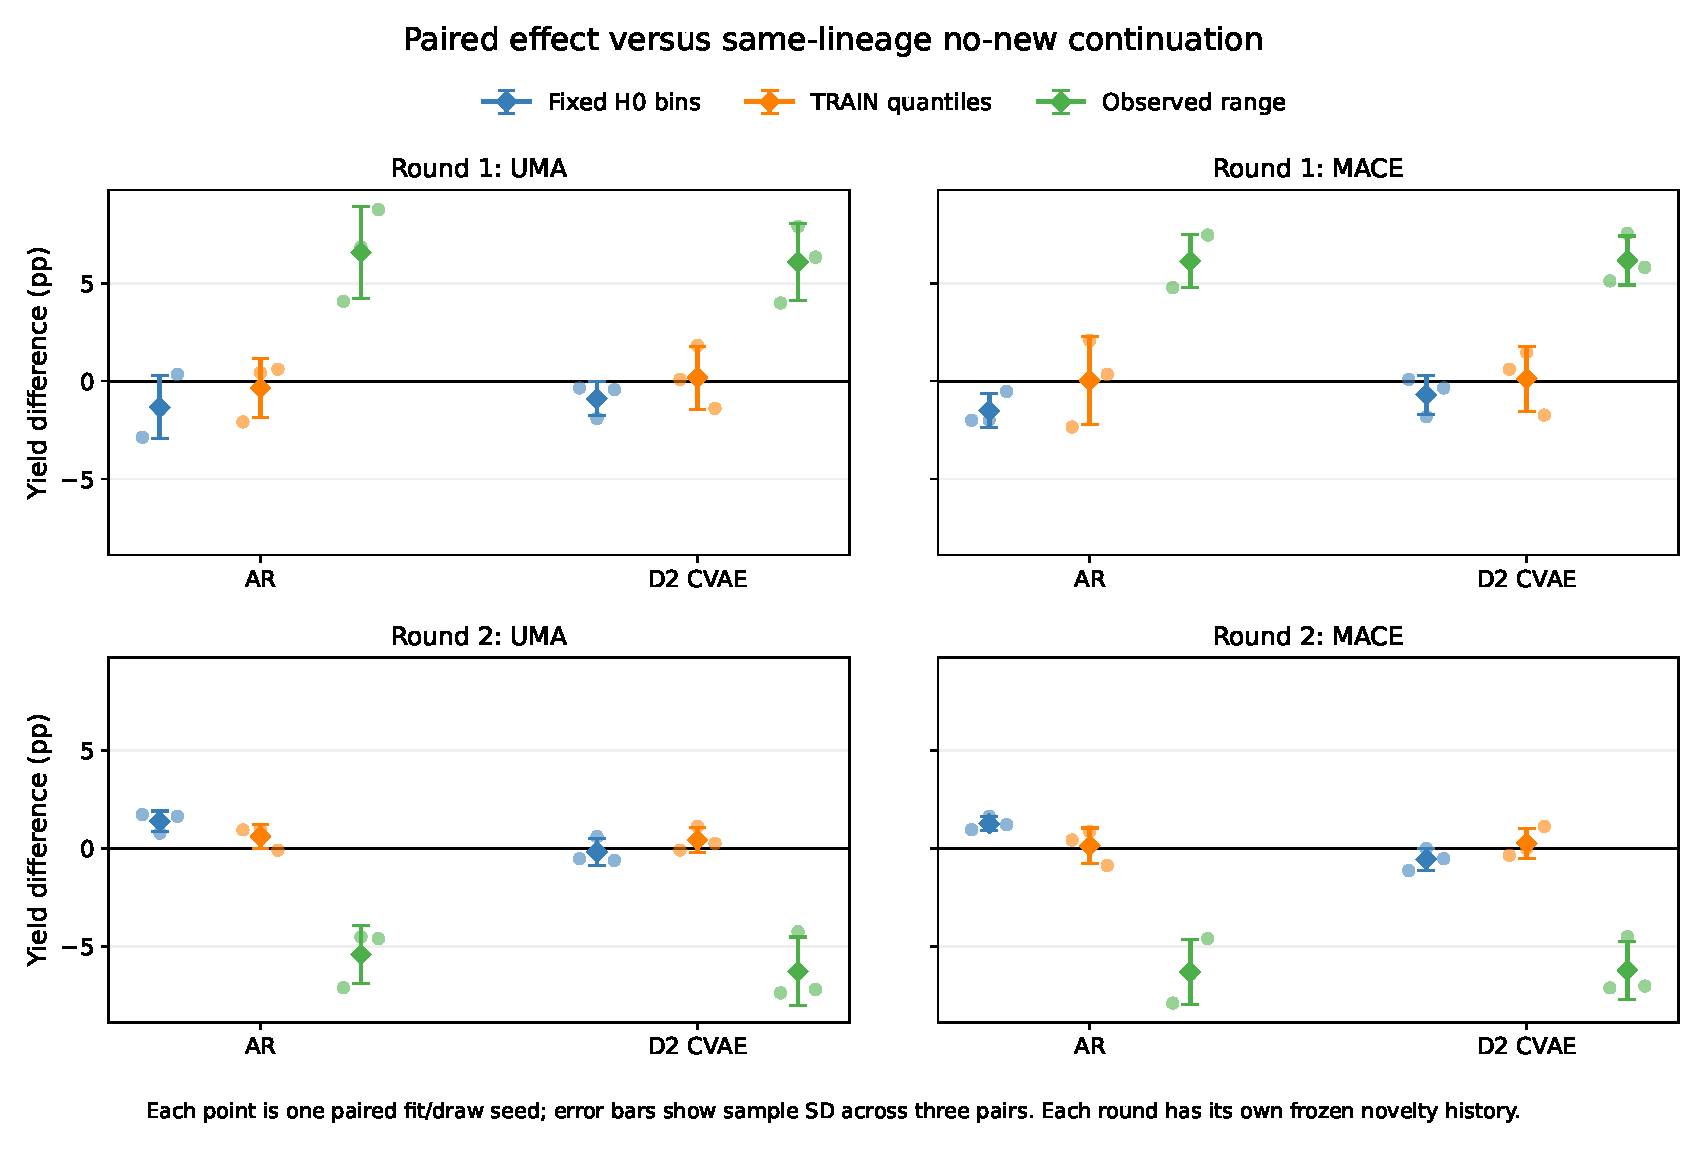
\includegraphics[width=\linewidth]{iteration_paired_gains.pdf}
\caption{Acquisition effects within separately frozen assessments. Each
round uses its appropriate no-new-data continuation; round 2 starts both
arms from the same first-round lineage. Error bars are SD over three paired
fit/proposal seeds.}
\end{figure}

After round two, absolute UMA range yields remain 70.28\% for AR and
68.66\% for $D=2$, above the declared fresh uniform and fixed-TRAIN-seed
mutation baselines of $33.88\pm0.59$\% and $58.16\pm1.53$\%. Nevertheless,
continuing the first-round model without the new range batch performs better.
The decline mainly appears in fixed-bin condition fidelity; novelty still
exceeds 97\%.

This requires care in interpretation. Acquiring higher-energy extrema raises
the range-defined LOW cutoff, so the requested target itself becomes less
strict relative to the fixed-H0 LOW reference. The negative fixed-metric
change and the positive extension of upper-energy coverage describe different
outcomes. The detailed report separates novelty, condition fidelity, moving
bins, endpoint growth, and loss-weight concentration rather than reducing
them to one success label.

\begin{table}[htbp]
\centering\small
\caption{Posthoc conditioning/data controls: balanced H0 fixed-bin yield change, percentage points, mean $\pm$ sample SD over three paired fits. Relabeling also changes class-balanced loss weights. The matched-range comparison holds the physical edges identical; adding rows can still change minibatches and row weights.}
\begin{tabular}{lrr}\toprule
Model / contrast & UMA & MACE\\\midrule
AR / H0 range versus fixed & $+6.48\pm1.01$ & $+6.11\pm0.98$\\
AR / New rows / fixed edges & $-1.56\pm0.88$ & $-1.10\pm1.33$\\
AR / New rows / matched range edges & $-1.36\pm0.39$ & $-2.05\pm0.84$\\
CVAE $D=2$ / H0 range versus fixed & $+7.06\pm1.09$ & $+6.80\pm0.91$\\
CVAE $D=2$ / New rows / fixed edges & $+0.41\pm0.78$ & $+0.09\pm0.46$\\
CVAE $D=2$ / New rows / matched range edges & $+1.85\pm1.33$ & $+2.00\pm1.39$\\
\bottomrule\end{tabular}
\end{table}


A fresh, explicitly post-hoc control shows that most of the first-round
range-label gain does not require new structures. Starting from the same
original checkpoint and allocating the same 2,000-update continuation,
relabeling H0 alone improves balanced UMA yield by $6.48\pm1.01$ points for
AR and $7.06\pm1.09$ for $D=2$. Independent MACE assessment gives
$6.11\pm0.98$ and $6.80\pm0.91$ points. At identical first-round range edges,
adding the acquired rows instead changes UMA yield by $-1.36\pm0.39$ points
for AR and $+1.85\pm1.33$ for $D=2$; MACE gives $-2.05\pm0.84$ and
$+2.00\pm1.39$ points. These are three-pair sample SDs.

The larger improvement is therefore available through conditioning and its
associated loss reweighting on existing data. The smaller added-row effect
depends on architecture. This does not negate the measured expansion of
upper-energy samples: fixed-bin fidelity and exploration of a wider observed
energy range answer different questions. Neither outcome establishes DFT
accuracy, physical stability, or global coverage.



\section{Does the latent vector add useful physical control?}
We test latent dimensions $D=1,2,4$, a cyclic KL schedule \cite{fu}, and genuine, condition-only,
and shuffled physical-target heads. During training the encoder supplies a
mean $\mu$ and standard deviation $\sigma$, and samples
$z=\mu+\sigma\odot\epsilon$ with $\epsilon\sim\mathcal N(0,I)$, multiplying
coordinates element by element.
Generation uses a standard-normal prior without an input mask. The
Kullback--Leibler (KL) penalty encourages agreement between these latent
distributions. The target $C_{\rm vv}$ is the fraction
of nearest-neighbor periodic edges whose two sites are vacant. It describes
local vacancy clustering. The auxiliary target is centered and scaled using
TRAIN data within each composition--energy-bin cell, so conditions alone
cannot explain its mean variation. Genuine-head weights 1, 10, and 100,
plus supervision of the posterior mean instead of its noisy sample, are
tested with matched controls. The latent studies complete 85 fits, all at
4,000 updates and five seeds per family. These matched budgets do not
certify full optimizer convergence; the detailed report retains loss curves.

\begin{table}[htbp]
\centering\small
\caption{Primary balanced novel correct-bin yield, percent, mean $\pm$ sample SD over five fit/proposal seeds. Compare arms within this phase's fresh development history.}
\begin{tabular}{lrr}\toprule
Model & UMA & MACE\\\midrule
AR & $62.92\pm1.41$ & $63.82\pm0.99$\\
CVAE $D=1$ & $63.12\pm1.40$ & $63.68\pm0.75$\\
CVAE $D=2$ & $62.76\pm0.60$ & $63.49\pm1.38$\\
CVAE $D=4$ & $63.39\pm1.75$ & $64.03\pm0.41$\\
\bottomrule\end{tabular}
\end{table}


None of these latent interventions establishes a primary sampling advantage
over AR. On a separate fresh assessment, mean supervision gives
$63.33\pm1.76$\% UMA yield versus $63.47\pm0.86$\% for AR, with five-fit
sample SD. Genuine guidance does not reliably move the actual generated
vacancy-pair fraction in its requested direction; shuffled heads can move it
as much or more. A small positive contrast under stronger supervision is
retained in the detailed report, together with its unsuccessful AR and
shuffled-target comparisons.

The representation contains more information than the original pooled probe
suggested. A posthoc probe, standardized and fitted separately within each
condition using TRAIN only, recovers clustering from VAL posterior means.
Balanced MSE is $0.1009\pm0.0963$ for $D=2$, versus 1.0212 for the zero
reference. Yet random graph initialization recovers this property even more
accurately in the fixed-condition control: physical graph structure already
provides useful features before training.

This does not give useful sampled-latent control. In one predeclared
24-Li/MIDDLE illustration, variations of the mean are roughly
$10^{-6}$--$10^{-8}$, whereas posterior sampling noise has standard deviation
about one. An analytic Gaussian-mixture calculation bounds information
distinguishing the 986 empirical VAL records in noisy $Z$ below
$10^{-10}$ nats for the three illustrated fits. This concerns the encoder
joint in one condition; prior-decoder interventions are a separate test.
The detailed report supplies the derivation, high-precision checks, and
corrected mean/noise plots. A colored mean scatter alone would therefore
overstate useful physical information in generated samples.

\section{Entropy: weighting the proposal for a different task}
Novel-structure search and entropy estimation use different counting rules.
For a new idealized 12-site O3 lattice, exhaustive enumeration gives 4,096
labelled occupancies and 87 symmetry orbits. At half occupancy, 924 labelled
masks form only 17 orbits. If orbit $o$ represents $g_o$ masks, its thermal
weight must include $g_o$:
\begin{equation}
Z_{\rm rel}=\sum_o g_o e^{-\epsilon_o/(\kb T)},\qquad
S/\kb=\log Z_{\rm rel}+\langle\epsilon\rangle/(\kb T).
\end{equation}
$\epsilon_o=E_o-E_{\min}$ is total energy per cell in eV, $T$ is K, and
$\kb$ is Boltzmann's constant. This is finite-cell configurational entropy;
vibrations, spin states, phase changes, and cell-size transfer are excluded.
Each teacher evaluates 87 representatives plus 36 symmetry checks. The exact
reference expands representative energies by multiplicity. Measured numerical
symmetry errors, particularly UMA at low temperature, qualify this assumption.

A learned proposal $q(x)$ is not automatically a thermal distribution.
Importance sampling divides each Boltzmann factor by the actual proposal
probability \cite{owen}. Weight effective sample size (ESS),
$(\sum_mw_m)^2/\sum_mw_m^2$, measures concentration of importance weights
$w_m$; $M$ is the number of draws. We use exact AR probabilities and a 10\% uniform
mixture to guarantee support, retain repeated masks, and compare against the
complete small-lattice reference. The original composition-only AR is less
efficient than uniform in the main comparison. A follow-up instead trains
three same-seed AR models per teacher using TRAIN weights proportional to
$g_o\exp[-E_o/(\kb\times1000\,\mathrm K)]$, normalized to preserve each
composition's original TRAIN weight mass. No held-out energy affects these
weights; TEST energies remain NaN in learning exports.

\begin{table}[htbp]
\centering\small
\caption{Temperature transfer of the 1,000 K-trained proposal. Entries are descriptive equal-composition averages over $n=3,6,9$ at 8,192 draws; MAE is in $k_{\rm B}$ per cell and ESS/$M$ is dimensionless. They are not averages of a physical entropy across compositions.}
\begin{tabular}{llrrrrr}\toprule
Teacher & $T$ (K) & AR MAE & Weighted MAE & Uniform MAE & W. ESS/$M$ & U. ESS/$M$\\\midrule
UMA & 300 & 0.026879 & 0.008345 & 0.020461 & 0.3038 & 0.1044\\
UMA & 1000 & 0.013095 & 0.004204 & 0.009409 & 0.7296 & 0.2495\\
UMA & 5000 & 0.001973 & 0.008512 & 0.001763 & 0.6274 & 0.8259\\
MACE & 300 & 0.020480 & 0.005252 & 0.016783 & 0.6374 & 0.2549\\
MACE & 1000 & 0.013710 & 0.003133 & 0.011170 & 0.7420 & 0.3006\\
MACE & 5000 & 0.001984 & 0.009692 & 0.001704 & 0.6515 & 0.8267\\
\bottomrule\end{tabular}
\end{table}


At 1,000 K, target weighting improves measured mean absolute entropy error
(MAE) and weight ESS
for all three tested compositions, but the same proposal performs worse than
uniform at 5,000 K. The table reports descriptive averages across the three
compositions, rather than a physical average entropy. Three fits and three
draw seeds per fit provide the sampling comparisons. These draws reuse the
tabulated energies, so they benchmark estimator error rather than additional
MLIP cost. A CVAE would require its latent-marginal proposal probability;
the decoder likelihood at one latent sample is insufficient for this weight.

There is also an important negative numerical result. All 36 bounded
Wang--Landau runs \cite{wanglandau} meet their specified schedule, but UMA's
Li6/12 entropy at 300 K changes materially with energy-bin resolution:
the exact discrete value is 3.26849\,$\kb$, versus exact midpoint-binned
values 4.34857 and 3.51230 for 16 and 32 bins. Completing a flat-histogram
schedule has not established bin-width convergence.

\section{Decisions, reproducibility, and collaborator tasks}
Retain AR as the reference generator and treat range relabeling as a
conditioning/reweighting policy. Its gain does not establish that another
acquired batch is beneficial, or that LOW requests improve as much as HIGH
requests. Future comparisons should preserve a common assessment history
and separate fixed-bin fidelity from extension of the observed range.

The next latent test should target information that survives posterior
sampling and produces a directed change in generated structures. Recovering
ordering from tiny encoder-mean variations is useful diagnosis, but does not
establish that the learned latent improves generation. The entropy study
likewise shows why the sampling objective matters: its 1,000\,K proposal
helps that target but loses to uniform sampling at 5,000\,K.

\begin{itemize}[leftmargin=*,itemsep=3pt]
\item \textbf{Ricardo} reviews endpoint structures, symmetry and units,
interprets teacher disagreements, and defines later DFT/relaxation checks.
\item \textbf{Beihao} reproduces AR/CVAE training and develops a controlled
sampled-latent test with the existing data, matched budgets, and genuine,
condition-only, shuffled and random-encoder comparisons.
\item \textbf{Varad} reproduces the paired evaluations, audits thresholds
and denominators, reports per-cell variability and negative results, and
maintains the analysis and cost receipts.
\end{itemize}

Independent DFT accuracy, relaxed structures, non-O3 phases, size transfer,
and stable dynamics remain physical validation tasks. The current
fixed-lattice MLIP results do not establish those outcomes.


The integrated package checks pass 414 tests, with six skips. Full task
arguments, checkpoint/input hashes, raw proposals, exclusions, failed
technical attempts, teacher receipts, and assessment boundaries remain in
the run archive. The accompanying detailed report and compact evidence
packet provide the numerical tables, derivations, figures, commands, and
cost definitions. Neural/MLIP computation uses FP32 with TF32 disabled;
entropy sums and moment diagnostics use float64. No new DFT, MD, or MLIP
fine-tuning is performed.
The campaign completes 166 generative fits (520,000 optimizer updates) and
469,672 geometry--teacher static evaluations, including repeat evaluations
required by separately frozen comparisons. This is an evaluation-event count,
not the number of globally unique physical geometries. The final allocation
receipt reports all four Slurm allocations, including startup, idle time and
failed technical subprocesses, with GPU-node-hours defined as allocated
GPU-device hours divided by four. Shared-node allocations can overlap on the
same physical node. This estimate is distinct from an official posted charge;
the compact packet's \texttt{resource\_receipt.json} records final
usage of 28.8799 GPU-node-hours (115.5194 allocated
GPU-device hours), below the 150 GPU-node-hour limit. All four allocations
have ended; three idle allocations were explicitly released and the final
shared workers exited normally.


\begin{thebibliography}{9}
\bibitem{uma} B. M. Wood et al.
UMA: A Family of Universal Models for Atoms (2025).
\url{https://arxiv.org/abs/2506.23971}.
\bibitem{macefoundation} MACE developers.
Foundation models: MACE-MH-1/0. Official model documentation,
accessed November 13, 2026.
\url{https://mace-docs.readthedocs.io/en/latest/guide/foundation_models.html}.
\bibitem{wakamiya} T. Wakamiya and A. Ishikawa.
Artificial catalyst generation for the oxygen reduction reaction using
conditional variational autoencoder and atomistic calculations.
\emph{npj Computational Materials} 12, 206 (2026).
\url{https://doi.org/10.1038/s41524-026-02075-0}.
\bibitem{kingma} D. P. Kingma and M. Welling.
Auto-Encoding Variational Bayes. ICLR (2014).
\url{https://arxiv.org/abs/1312.6114}.
\bibitem{fu} H. Fu et al.
Cyclical Annealing Schedule: A Simple Approach to Mitigating KL Vanishing.
NAACL-HLT, 240--250 (2019).
\url{https://doi.org/10.18653/v1/N19-1021}.
\bibitem{wanglandau} F. Wang and D. P. Landau.
Efficient, Multiple-Range Random Walk Algorithm to Calculate the Density of
States. \emph{Physical Review Letters} 86, 2050--2053 (2001).
\url{https://doi.org/10.1103/PhysRevLett.86.2050}.
\bibitem{owen} A. B. Owen.
\emph{Monte Carlo theory, methods and examples}, Chapter 9,
Sections 9.1--9.3 (2013).
\url{https://artowen.su.domains/mc/Ch-var-is.pdf}.
\end{thebibliography}

\end{document}
